% ============================================================
%  Module 3 — Malthus and Ricardo
%  From Smith to Simulation · University of Edinburgh
% ============================================================
\documentclass[aspectratio=169, 10pt]{beamer}
\usetheme{metropolis}

% --- Edinburgh colours ----------------------------------------
\definecolor{UoERed}{HTML}{7A2318}
\definecolor{UoEGold}{HTML}{B8860B}
\definecolor{CodeBG}{HTML}{F7F3ED}
\definecolor{CodeFrame}{HTML}{D5C9B1}

\setbeamercolor{palette primary}{bg=UoERed, fg=white}
\setbeamercolor{frametitle}{bg=UoERed, fg=white}
\setbeamercolor{title separator}{fg=UoEGold}
\setbeamercolor{progress bar}{fg=UoEGold, bg=UoEGold!20}
\setbeamercolor{alerted text}{fg=UoERed}
\setbeamercolor{block title}{bg=UoERed!15, fg=UoERed}
\setbeamercolor{block body}{bg=UoERed!5}

% --- Packages -------------------------------------------------
\usepackage[T1]{fontenc}
\usepackage{lmodern}
\usepackage{amsmath, amssymb, mathtools}
\usepackage{listings}
\usepackage{graphicx, booktabs}
\usepackage{tikz}
\usetikzlibrary{arrows.meta, positioning, calc, decorations.pathreplacing}
\usepackage{hyperref}
\hypersetup{colorlinks=true, linkcolor=UoERed, urlcolor=UoERed!70!black}
\setbeamertemplate{navigation symbols}{}

\lstset{
  language=Python,
  basicstyle=\ttfamily\scriptsize,
  keywordstyle=\color{UoERed}\bfseries,
  commentstyle=\color{gray}\itshape,
  stringstyle=\color{UoEGold},
  backgroundcolor=\color{CodeBG},
  frame=single,
  rulecolor=\color{CodeFrame},
  numbers=none,
  breaklines=true,
  showstringspaces=false,
  tabsize=4,
  xleftmargin=4pt, xrightmargin=4pt,
  aboveskip=6pt, belowskip=4pt,
}

% Section title pages
\AtBeginSection[]{
  \begin{frame}
    \vfill\centering
    \usebeamerfont{title}\insertsectionhead\par
    \vfill
  \end{frame}
}

% ---- Title ---------------------------------------------------
\title{Module 3 --- Malthus and Ricardo}
\subtitle{Population, Land, and the Limits to Growth}
\author{Dr Juan Zurita}
\institute{From Smith to Simulation\\
The University of Edinburgh~$\cdot$~School of Economics}
\date{}

\begin{document}

% =============================================================
\maketitle
% =============================================================

% -------------------------------------------------------------
\section{Part I --- The History}
% -------------------------------------------------------------

\begin{frame}{London, 1798}
\begin{columns}[T]
\column{0.55\textwidth}
\begin{itemize}
  \item Twenty-two years after Smith's optimistic vision, a young
        English clergyman publishes\\
        \textit{An Essay on the Principle of Population}.
  \item \textbf{Thomas Robert Malthus} (1766--1834) argued
        that humanity was \alert{trapped}.
  \item One of the most influential --- and controversial --- books
        in the history of social science.
\end{itemize}
\column{0.4\textwidth}
\begin{block}{The Core Argument}
  Population, when unchecked, grows \textbf{geometrically}.
  Food production can only grow \textbf{arithmetically}.
  Therefore, population will always tend to outrun the food supply.
\end{block}
\end{columns}
\end{frame}

\begin{frame}{The Darkest Idea in Economics}
\begin{center}
\textit{``The power of population is indefinitely greater than the\\
power in the earth to produce subsistence for man.''}\\[4pt]
--- Thomas Malthus, \textit{Essay on the Principle of Population} (1798), Ch.~1
\end{center}
\vspace{1em}
Malthus's logic was brutally simple:
\begin{enumerate}
  \item \textbf{Population} grows \alert{geometrically} (exponentially) ---
        each generation is larger than the last.
  \item \textbf{Food production} grows only \alert{arithmetically} (linearly) ---
        there is only so much land.
  \item The result is misery: famine, disease, and war keep population
        in check.
\end{enumerate}
\end{frame}

\begin{frame}{Geometric vs Arithmetic Growth}
\begin{center}
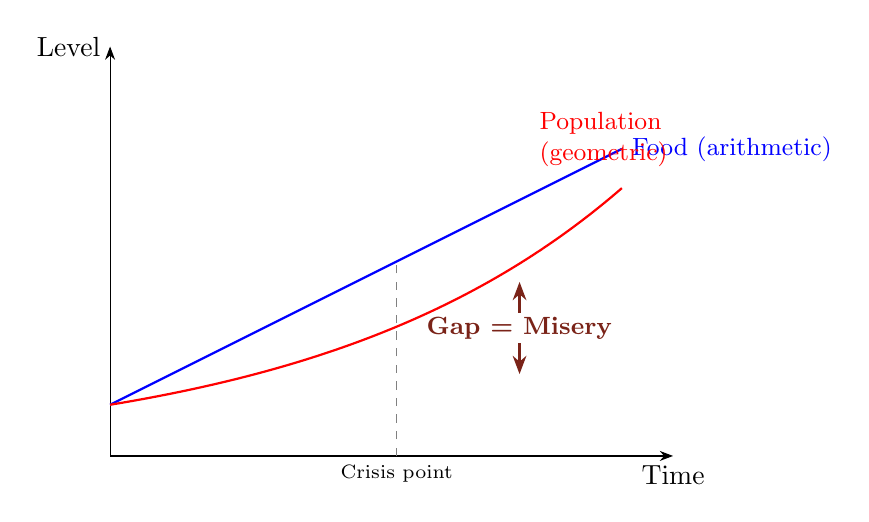
\begin{tikzpicture}[scale=0.65, >=Stealth]
  % Axes
  \draw[->] (0,0) -- (11,0) node[below] {Time};
  \draw[->] (0,0) -- (0,8) node[left] {Level};
  % Arithmetic growth (food): y = 1 + 0.5*t
  \draw[thick, blue] plot[smooth, domain=0:10, samples=50]
    (\x, {1 + 0.5*\x}) node[right, font=\small] {Food (arithmetic)};
  % Geometric growth (population): y = 1.0 * 1.15^t  scaled
  \draw[thick, red] plot[smooth, domain=0:10, samples=50]
    (\x, {1.0 * (1.18)^\x / 1.0})
    node[right, font=\small] {};
  \node[right, font=\small, red] at (8.2, 6.5) {Population};
  \node[right, font=\small, red] at (8.2, 5.9) {(geometric)};
  % Intersection area
  \draw[dashed, gray] (5.6, 0) -- (5.6, 3.8);
  \node[below, font=\scriptsize] at (5.6, 0) {Crisis point};
  % Shaded region label
  \node[font=\small, UoERed] at (8, 2.5) {\textbf{Gap = Misery}};
  \draw[->, UoERed, thick] (8, 2.8) -- (8, 3.4);
  \draw[->, UoERed, thick] (8, 2.2) -- (8, 1.6);
\end{tikzpicture}
\end{center}
\vspace{0.3em}
Population growth eventually \textbf{outstrips} food production.\\
The gap is closed by what Malthus called ``positive checks'': famine, disease, war.
\end{frame}

\begin{frame}{The Dismal Science}
\begin{block}{Why Economics Earned Its Nickname}
  Thomas Carlyle called economics \textit{``the dismal science''} ---
  the phrase was aimed at the gloomy predictions of Malthus and his followers.
\end{block}
\vspace{0.5em}
\begin{itemize}
  \item Smith (1776) was \textbf{optimistic}: markets create wealth for all.
  \item Malthus (1798) was \textbf{pessimistic}: population devours any gains.
  \item Wages are forever pulled back to \alert{subsistence}.
  \item No amount of charity or good intentions can change this ---
        it is a law of nature.
\end{itemize}
\vspace{0.5em}
For most of human history, \textbf{Malthus was right}.
\end{frame}

\begin{frame}{Was Malthus Right? The Malthusian Trap}
\begin{columns}[T]
\column{0.55\textwidth}
\begin{itemize}
  \item For \textbf{thousands of years} before the Industrial Revolution,
        living standards barely changed.
  \item When agricultural productivity improved --- a new crop,
        a better plough --- the result was not richer people but
        \textit{more} people.
  \item Population expanded until it pressed against
        the food supply, and wages returned to subsistence.
  \item Gregory Clark (\textit{A Farewell to Alms}, 2007):
        the average English person in 1800 was no better off
        than in 100,000~BC.
\end{itemize}
\column{0.4\textwidth}
\begin{alertblock}{The Trap}
  Any surplus is eaten up (literally) by population growth.
  Better technology $\Rightarrow$ more people, \textbf{not} richer people.
\end{alertblock}
\vspace{0.5em}
Then, around 1800, something extraordinary happened\ldots
\end{columns}
\end{frame}

\begin{frame}{David Ricardo and Diminishing Returns}
\begin{columns}[T]
\column{0.55\textwidth}
Malthus's friend and sparring partner,
\textbf{David Ricardo} (1772--1823), formalised the mechanism:
\vspace{0.3em}
\begin{itemize}
  \item As more labour is applied to \textbf{fixed land},
        each additional worker produces \textit{less} additional output.
  \item First farmers clear the best land; then the second-best;
        eventually, rocky hillsides.
  \item This is why food production can't keep up --- not because
        farming doesn't improve, but because the \alert{marginal}
        improvement gets smaller.
\end{itemize}
\column{0.4\textwidth}
\begin{center}
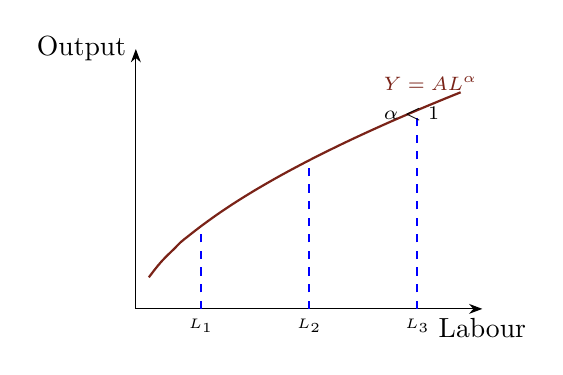
\begin{tikzpicture}[scale=0.55, >=Stealth]
  \draw[->] (0,0) -- (8,0) node[below] {Labour};
  \draw[->] (0,0) -- (0,6) node[left] {Output};
  % Diminishing returns curve
  \draw[thick, UoERed] plot[smooth, domain=0.3:7.5, samples=50]
    (\x, {5 * (\x/7.5)^0.6});
  % Tangent lines showing diminishing MPL
  \draw[dashed, blue, thick] (1.5, 0) -- (1.5, {5*(1.5/7.5)^0.6});
  \draw[dashed, blue, thick] (4.0, 0) -- (4.0, {5*(4.0/7.5)^0.6});
  \draw[dashed, blue, thick] (6.5, 0) -- (6.5, {5*(6.5/7.5)^0.6});
  \node[below, font=\tiny] at (1.5, 0) {$L_1$};
  \node[below, font=\tiny] at (4.0, 0) {$L_2$};
  \node[below, font=\tiny] at (6.5, 0) {$L_3$};
  % Brace for diminishing increments
  \node[right, font=\scriptsize, UoERed] at (5.5, 5.2) {$Y = A L^\alpha$};
  \node[right, font=\scriptsize] at (5.5, 4.5) {$\alpha < 1$};
\end{tikzpicture}
\end{center}
\end{columns}
\end{frame}

\begin{frame}{Ricardo's Income Distribution}
Ricardo showed how diminishing returns determined the
\textbf{distribution of income}:
\vspace{0.5em}
\begin{columns}[T]
\column{0.48\textwidth}
\begin{block}{Workers}
  Receive \textbf{wages} $= $ marginal product of labour.\\
  As population grows, wages \textit{fall} toward subsistence.
\end{block}
\column{0.48\textwidth}
\begin{block}{Landlords}
  Receive \textbf{rents} $= Y - wL$.\\
  As population grows, rents \textit{rise} --- landlords capture
  an increasing share.
\end{block}
\end{columns}
\vspace{1em}
\begin{center}
Population growth $\Rightarrow$ workers \textit{worse off},
landlords \textit{better off}.\\[4pt]
A grim picture --- and Marx would later build on it.
\end{center}
\end{frame}

\begin{frame}{Edinburgh and the Scottish Connection}
\begin{itemize}
  \item Malthus's \textit{Essay} was partly a response to Enlightenment optimists
        (Condorcet, Godwin) who believed humanity was perfectible.
  \item Malthus --- educated in the Scottish tradition of empirical argument ---
        responded with \textbf{data and logic} rather than hope.
  \item \textbf{Dugald Stewart}, who held Adam Smith's old chair
        of moral philosophy at Edinburgh, disseminated both Smith's
        and Malthus's ideas to the next generation.
  \item The Scottish Enlightenment's commitment to
        \alert{following evidence wherever it leads}, even to uncomfortable
        conclusions, is visible throughout Malthus's work.
\end{itemize}
\end{frame}

% -------------------------------------------------------------
\section{Part II --- The Computation}
% -------------------------------------------------------------

\begin{frame}[fragile]{Setting Up}
\begin{lstlisting}
import numpy as np
import matplotlib.pyplot as plt
\end{lstlisting}
\vspace{0.5em}
\begin{itemize}
  \item \texttt{numpy} --- numerical arrays and operations
  \item \texttt{matplotlib} --- plotting
\end{itemize}
\vspace{0.5em}
We will build and simulate the Malthusian model step by step,
then watch it \textbf{reproduce ten thousand years of economic history}.
\end{frame}

\begin{frame}{The Production Function: Diminishing Returns}
Following Ricardo, we model food production with a
\textbf{Cobb--Douglas production function} where land is fixed:
\[
  Y = A \cdot L^{\alpha}
\]
\begin{itemize}
  \item $Y$ = total food output
  \item $L$ = population (= labour force in this pre-industrial world)
  \item $A$ = productivity parameter (quality of seeds, techniques)
  \item $\alpha \in (0,1)$ captures \alert{diminishing returns}
\end{itemize}
\vspace{0.5em}
The crucial feature: $\alpha < 1$ means doubling the population
does \textit{not} double food production.\\[4pt]
This is Ricardo's diminishing returns, expressed mathematically.
\end{frame}

\begin{frame}[fragile]{Production Function in Python}
\begin{lstlisting}
# Parameters
A = 10       # productivity
alpha = 0.6  # diminishing returns (less than 1)

def production(L, A=A, alpha=alpha):
    """Total food output given population L."""
    return A * L**alpha

def output_per_capita(L, A=A, alpha=alpha):
    """Food per person = Y/L = A * L^(alpha-1)."""
    return A * L**(alpha - 1)
\end{lstlisting}
\vspace{0.3em}
\begin{columns}[T]
\column{0.48\textwidth}
\textbf{Total output} rises with $L$\ldots
\column{0.48\textwidth}
\ldots but \textbf{output per person} falls.
\end{columns}
\vspace{0.3em}
This is the essence of the Malthusian trap.
\end{frame}

\begin{frame}{Diminishing Returns: The Picture}
\begin{center}
\begin{tikzpicture}[scale=0.55, >=Stealth]
  % Left panel: Total output
  \begin{scope}
    \draw[->] (0,0) -- (7,0) node[below] {$L$};
    \draw[->] (0,0) -- (0,5.5) node[left] {$Y$};
    \draw[thick, UoERed] plot[smooth, domain=0.2:6.5, samples=50]
      (\x, {4.5 * (\x/6.5)^0.6});
    \node[above, font=\small] at (3.5, 5.5) {Total Output $Y = AL^\alpha$};
    \node[right, font=\scriptsize, UoERed] at (5.5, 4.2) {concave};
  \end{scope}
  % Right panel: Output per capita
  \begin{scope}[xshift=9cm]
    \draw[->] (0,0) -- (7,0) node[below] {$L$};
    \draw[->] (0,0) -- (0,5.5) node[left] {$Y/L$};
    \draw[thick, blue] plot[smooth, domain=0.4:6.5, samples=50]
      (\x, {4.5 * (\x/6.5)^(-0.4)});
    % Subsistence line
    \draw[dashed, black] (0, 1.2) -- (7, 1.2);
    \node[right, font=\scriptsize] at (5.5, 1.5) {$\bar{c}$};
    \node[above, font=\small] at (3.5, 5.5) {Per Capita $Y/L = AL^{\alpha-1}$};
    \node[right, font=\scriptsize, blue] at (4.5, 3.0) {falling};
  \end{scope}
\end{tikzpicture}
\end{center}
\vspace{0.3em}
As population grows, total output rises but each person gets \textbf{less}.\\
Eventually, output per capita hits the subsistence level $\bar{c}$.
\end{frame}

\begin{frame}{Population Dynamics: The Malthusian Mechanism}
Malthus's key insight: population growth \textit{responds} to living standards.
\vspace{0.3em}
\[
  L_{t+1} = L_t \cdot \bigl(1 + g\,(y_t - \bar{c})\bigr)
\]
\vspace{0.3em}
where $y_t = Y_t / L_t$ is food per person.
\vspace{0.5em}
\begin{itemize}
  \item $y > \bar{c}$: plenty of food $\Rightarrow$ population \textbf{grows}
        (more children, fewer deaths).
  \item $y < \bar{c}$: famine $\Rightarrow$ population \textbf{shrinks}
        (fewer children, more deaths).
  \item $y = \bar{c}$: population is \textbf{stable} --- the
        \alert{Malthusian steady state}.
\end{itemize}
\end{frame}

\begin{frame}{The Feedback Loop}
\begin{center}
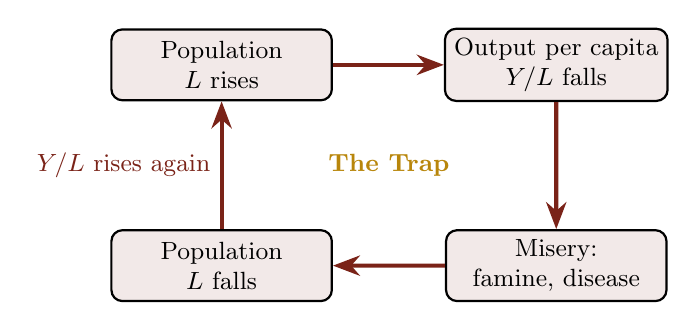
\begin{tikzpicture}[>=Stealth, thick, scale=0.85,
  box/.style={draw, rounded corners, fill=UoERed!10,
              minimum width=2.8cm, minimum height=0.9cm,
              font=\small, align=center}]
  \node[box] (pop) at (0, 0) {Population\\$L$ rises};
  \node[box] (ypc) at (5, 0) {Output per capita\\$Y/L$ falls};
  \node[box] (mis) at (5, -3) {Misery:\\famine, disease};
  \node[box] (dec) at (0, -3) {Population\\$L$ falls};
  \draw[->, line width=1.5pt, UoERed] (pop) -- (ypc);
  \draw[->, line width=1.5pt, UoERed] (ypc) -- (mis);
  \draw[->, line width=1.5pt, UoERed] (mis) -- (dec);
  \draw[->, line width=1.5pt, UoERed] (dec) --
    node[left, font=\small] {$Y/L$ rises again} (pop);
  \node[font=\small\bfseries, UoEGold] at (2.5, -1.5) {The Trap};
\end{tikzpicture}
\end{center}
\vspace{0.5em}
A self-correcting system --- but one that corrects through \textbf{suffering}.
\end{frame}

\begin{frame}[fragile]{Simulating the Malthusian Model}
\begin{lstlisting}
c_bar = 1.5    # subsistence consumption
g = 0.02       # population growth sensitivity
T = 300        # number of periods
L0 = 50        # initial population

def simulate_malthus(L0, A, alpha, c_bar, g, T):
    L = np.empty(T)
    y = np.empty(T)
    L[0] = L0
    y[0] = A * L0**(alpha - 1)

    for t in range(1, T):
        growth_rate = g * (y[t-1] - c_bar)
        L[t] = max(L[t-1] * (1 + growth_rate), 1)
        y[t] = A * L[t]**(alpha - 1)
    return L, y

L_sim, y_sim = simulate_malthus(L0, A, alpha, c_bar, g, T)
\end{lstlisting}
\end{frame}

\begin{frame}{Convergence to the Steady State}
\begin{center}
\begin{tikzpicture}[scale=0.65, >=Stealth]
  % Left panel: population
  \begin{scope}
    \draw[->] (0,0) -- (8,0) node[below] {Time};
    \draw[->] (0,0) -- (0,5.5) node[left] {$L$};
    % Population growing and levelling off
    \draw[thick, blue] plot[smooth] coordinates
      {(0,0.8) (1,1.2) (2,1.8) (3,2.6) (4,3.3) (5,3.9) (6,4.3) (7,4.5) (7.5,4.55)};
    \draw[dashed, black] (0, 4.55) -- (8, 4.55);
    \node[left, font=\scriptsize] at (0, 4.55) {$L^*$};
    \node[above, font=\small] at (4, 5.5) {Population};
  \end{scope}
  % Right panel: output per capita
  \begin{scope}[xshift=10cm]
    \draw[->] (0,0) -- (8,0) node[below] {Time};
    \draw[->] (0,0) -- (0,5.5) node[left] {$Y/L$};
    % y/L falling to subsistence
    \draw[thick, red] plot[smooth] coordinates
      {(0,4.5) (1,3.8) (2,3.0) (3,2.4) (4,2.0) (5,1.7) (6,1.55) (7,1.5) (7.5,1.5)};
    \draw[dashed, black] (0, 1.5) -- (8, 1.5);
    \node[left, font=\scriptsize] at (0, 1.5) {$\bar{c}$};
    \node[above, font=\small] at (4, 5.5) {Living Standards};
  \end{scope}
\end{tikzpicture}
\end{center}
\vspace{0.3em}
Population grows until output per capita falls to subsistence, then stabilises.\\[4pt]
\textbf{Living standards are trapped} --- exactly as Malthus predicted.
\end{frame}

\begin{frame}{Finding the Steady State Analytically}
At the Malthusian steady state, output per capita equals subsistence:
\[
  \frac{Y}{L} = A \cdot L^{\alpha - 1} = \bar{c}
\]
Solving for $L^*$:
\[
  \boxed{L^* = \left(\frac{A}{\bar{c}}\right)^{\!\frac{1}{1-\alpha}}}
\]
\vspace{0.3em}
\begin{itemize}
  \item Higher productivity $A$ $\Rightarrow$ \textbf{larger} steady-state population.
  \item But living standards are always $\bar{c}$ --- technology changes
        \textit{how many} people live at subsistence, not \textit{how well}.
\end{itemize}
\end{frame}

\begin{frame}[fragile]{Verifying the Steady State}
\begin{lstlisting}
def malthus_steady_state(A, alpha, c_bar):
    """Analytical steady-state population."""
    return (A / c_bar) ** (1 / (1 - alpha))

L_star = malthus_steady_state(A, alpha, c_bar)
print(f"Analytical L* = {L_star:.2f}")
print(f"Simulation L*  = {L_sim[-1]:.2f}")
\end{lstlisting}
\vspace{0.3em}
\begin{center}
\begin{tabular}{crc}
\toprule
$A$ & $L^*$ & Living standard \\
\midrule
 8  &  65.1 & $\bar{c} = 1.5$ \\
10  & 128.3 & $\bar{c} = 1.5$ \\
15  & 407.6 & $\bar{c} = 1.5$ \\
20  & 928.3 & $\bar{c} = 1.5$ \\
\bottomrule
\end{tabular}
\end{center}
Better technology $\Rightarrow$ bigger population, \textbf{same} living standard.
\end{frame}

\begin{frame}{The Cruel Irony}
\begin{block}{Does Better Technology Help?}
  Suppose someone invents a better plough (higher $A$).
  You might expect everyone to become richer. But:
\end{block}
\vspace{0.3em}
\begin{enumerate}
  \item Higher $A$ $\Rightarrow$ output per capita temporarily rises above $\bar{c}$.
  \item Population grows in response.
  \item Output per capita falls back to $\bar{c}$.
  \item \alert{The only lasting effect is a larger population.}
\end{enumerate}
\vspace{0.5em}
This explains why China and India had the world's largest populations
for centuries but not the highest living standards --- productive
agriculture translated into \textit{more mouths} rather than
\textit{fuller plates}.
\end{frame}

\begin{frame}[fragile]{Simulating the Cruel Irony}
\begin{lstlisting}
for A_val, label in [(8,  'A=8  (poor tech)'),
                     (10, 'A=10 (baseline)'),
                     (15, 'A=15 (better plough!)')]:
    L_s, y_s = simulate_malthus(L0, A_val, alpha, c_bar, g, T)
    plt.plot(y_s, label=label)

plt.axhline(c_bar, color='k', linestyle='--', label='Subsistence')
plt.legend()
plt.title('Living Standards for Different Technologies')
plt.show()
\end{lstlisting}
\vspace{0.3em}
All three economies converge to the \textbf{same} subsistence level.\\
Better technology $\Rightarrow$ more people, \textbf{not} richer people.
\end{frame}

\begin{frame}{The Wage Function}
In a competitive labour market, the wage equals the
\textbf{marginal product of labour}:
\[
  w = MPL = \alpha \cdot A \cdot L^{\alpha - 1}
\]
\begin{columns}[T]
\column{0.48\textwidth}
\textbf{Total wages:}
\[ wL = \alpha \cdot Y \]
\column{0.48\textwidth}
\textbf{Total rents (to landlords):}
\[ Y - wL = (1 - \alpha) \cdot Y \]
\end{columns}
\vspace{0.5em}
As population grows:
\begin{itemize}
  \item The \textit{wage per worker} $w$ \textbf{falls}
        (diminishing returns).
  \item Total \textit{rents} $(1-\alpha)Y$ \textbf{rise}
        (more output, landlords' share is constant).
  \item Ricardo's conclusion: population growth benefits
        \alert{landlords} at the expense of \alert{workers}.
\end{itemize}
\end{frame}

\begin{frame}{Breaking the Trap: The Industrial Revolution}
The Malthusian model describes the pre-industrial world perfectly.\\
But after 1800, something changed.
\vspace{0.5em}

Model technological progress as continuous productivity growth:
\[
  A_t = A_0 \cdot e^{\gamma t}
\]
\begin{itemize}
  \item If $\gamma$ is small: population absorbs the gains $\Rightarrow$
        \textbf{still trapped}.
  \item If $\gamma$ is large enough: productivity outpaces population
        $\Rightarrow$ \alert{escape!}
\end{itemize}
\vspace{0.5em}
The question of \textit{why} this happened --- why in Britain,
why around 1800 --- remains one of the most debated questions
in economic history.
\end{frame}

\begin{frame}[fragile]{Simulating the Escape}
\begin{lstlisting}
def simulate_with_growth(L0, A0, alpha, c_bar, g, gamma, T):
    L = np.empty(T);  y = np.empty(T);  A_t = np.empty(T)
    L[0], A_t[0] = L0, A0
    y[0] = A0 * L0**(alpha - 1)
    for t in range(1, T):
        A_t[t] = A0 * np.exp(gamma * t)
        growth_rate = g * (y[t-1] - c_bar)
        L[t] = max(L[t-1] * (1 + growth_rate), 1)
        y[t] = A_t[t] * L[t]**(alpha - 1)
    return L, y, A_t
\end{lstlisting}
\vspace{0.3em}
Three scenarios:
\begin{itemize}
  \item $\gamma = 0$: no growth (pre-1800) $\Rightarrow$ trapped
  \item $\gamma = 0.003$: slow growth $\Rightarrow$ partially escapes
  \item $\gamma = 0.01$: Industrial Revolution $\Rightarrow$ \alert{full escape}
\end{itemize}
\end{frame}

\begin{frame}{The Great Escape}
\begin{center}
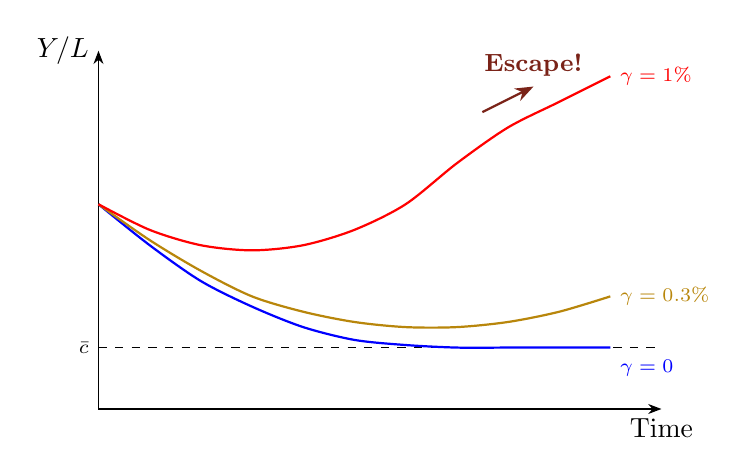
\begin{tikzpicture}[scale=0.65, >=Stealth]
  \draw[->] (0,0) -- (11,0) node[below] {Time};
  \draw[->] (0,0) -- (0,7) node[left] {$Y/L$};
  % Subsistence line
  \draw[dashed, black] (0, 1.2) -- (11, 1.2);
  \node[left, font=\scriptsize] at (0, 1.2) {$\bar{c}$};
  % No growth: converges to subsistence
  \draw[thick, blue] plot[smooth] coordinates
    {(0,4) (1,3.2) (2,2.5) (3,2.0) (4,1.6) (5,1.35) (6,1.25) (7,1.2) (8,1.2) (9,1.2) (10,1.2)};
  \node[right, font=\scriptsize, blue] at (10, 0.8) {$\gamma = 0$};
  % Slow growth: mostly stuck then slight rise
  \draw[thick, UoEGold] plot[smooth] coordinates
    {(0,4) (1,3.3) (2,2.7) (3,2.2) (4,1.9) (5,1.7) (6,1.6) (7,1.6) (8,1.7) (9,1.9) (10,2.2)};
  \node[right, font=\scriptsize, UoEGold] at (10, 2.2) {$\gamma = 0.3\%$};
  % Industrial Revolution: escapes
  \draw[thick, red] plot[smooth] coordinates
    {(0,4) (1,3.5) (2,3.2) (3,3.1) (4,3.2) (5,3.5) (6,4.0) (7,4.8) (8,5.5) (9,6.0) (10,6.5)};
  \node[right, font=\scriptsize, red] at (10, 6.5) {$\gamma = 1\%$};
  % Arrow
  \draw[->, thick, UoERed] (7.5, 5.8) -- (8.5, 6.3)
    node[above, font=\small\bfseries] {Escape!};
\end{tikzpicture}
\end{center}
\vspace{0.3em}
With fast enough technological progress, living standards
\textbf{break free from subsistence}.\\[4pt]
For 10,000 years the world was stuck. Then, in a few decades,
everything changed.
\end{frame}

% -------------------------------------------------------------
\section{Part III --- Exercises \& Discussion}
% -------------------------------------------------------------

\begin{frame}{Exercise 1: The Black Death (1348)}
The Black Death killed roughly \textbf{one-third} of Europe's population.
The Malthusian model makes a clear prediction.
\vspace{0.5em}
\begin{enumerate}
  \item Simulate the Malthusian model for 500~periods with
        $L_0 = 200$, $A = 10$, $\alpha = 0.6$, $\bar{c} = 1.5$,
        $g = 0.02$. Let it reach steady state.
  \item At period~250, kill one-third of the population
        (multiply $L$ by $2/3$). Continue the simulation.
  \item What happens to living standards \textit{immediately}
        after the plague? In the \textit{long run}?
  \item In 2--3 sentences, explain why a catastrophe that kills
        millions can \textit{improve} living standards for survivors.
\end{enumerate}
\vspace{0.3em}
\begin{block}{Historical evidence}
  Real wages in England roughly \textbf{doubled} after the Black Death.
\end{block}
\end{frame}

\begin{frame}{Exercise 2: Ricardo's Income Distribution}
With $Y = A \cdot L^\alpha$, the wage is $w = \alpha A L^{\alpha-1}$
and total rents are $(1-\alpha)Y$.
\vspace{0.5em}
\begin{enumerate}
  \item Compute and plot wage $w$ and total rents $(1-\alpha)Y$
        as functions of $L$ for $L \in [10, 500]$.
        Use $A = 10$, $\alpha = 0.6$.
  \item As population doubles from 100 to 200, what happens to
        individual wages? To total rents? Who benefits?
  \item Compute and plot the \textbf{rent-to-wage ratio}:
        \[
          \frac{(1-\alpha)\,Y}{\alpha \cdot A \cdot L^{\alpha-1}}
          = \frac{(1-\alpha)}{\alpha} \cdot L
        \]
        What happens as population grows?
\end{enumerate}
\end{frame}

\begin{frame}{Exercise 3: Carrying Capacity}
Modify the model to include an environmental
\textbf{carrying capacity}~$K$:
\[
  Y = A \cdot L^\alpha \cdot \left(1 - \frac{L}{K}\right)
\]
When $L$ approaches $K$, output drops to zero.
\vspace{0.5em}
\begin{enumerate}
  \item Simulate with $K = 500$, $A = 10$, $\alpha = 0.6$,
        $L_0 = 50$.
  \item What happens to the steady-state population and living
        standards compared to the basic model?
  \item Add technological progress ($\gamma = 0.005$).
        Does the economy still escape the trap? What is different?
\end{enumerate}
\vspace{0.3em}
\begin{alertblock}{Modern relevance}
  Some argue Malthusian dynamics apply today --- not for food, but for
  energy, water, and the atmosphere's capacity to absorb CO$_2$.
\end{alertblock}
\end{frame}

% -------------------------------------------------------------
\section{Quiz}
% -------------------------------------------------------------

\begin{frame}{Quiz: Conceptual Questions}
\begin{enumerate}
  \item Malthus argued population grows geometrically while food
        grows arithmetically. In modern terms:
        \begin{enumerate}
          \item[(a)] Population linear, food exponential
          \item[(b)] \alert{Population exponential, food linear}
          \item[(c)] Both at the same rate
          \item[(d)] Both exponential at different rates
        \end{enumerate}
  \item A one-time improvement in productivity (higher $A$) leads to:
        \begin{enumerate}
          \item[(a)] Permanently higher living standards
          \item[(b)] \alert{Temporarily higher, then back to subsistence
                     with larger population}
          \item[(c)] Lower living standards
          \item[(d)] No change
        \end{enumerate}
  \item Ricardo's ``diminishing returns'' means:
        \begin{enumerate}
          \item[(a)] Profits fall to zero
          \item[(b)] \alert{Each additional worker on fixed land produces
                     less additional output}
          \item[(c)] Wages always decrease
          \item[(d)] Trade produces diminishing benefits
        \end{enumerate}
\end{enumerate}
\end{frame}

\begin{frame}{Quiz: Computational Questions}
\begin{enumerate}
  \setcounter{enumi}{5}
  \item In $Y = A \cdot L^{0.6}$, if population doubles from 100 to 200,
        total output:
        \begin{enumerate}
          \item[(a)] Exactly doubles
          \item[(b)] More than doubles
          \item[(c)] \alert{Increases by $2^{0.6} \approx 1.52$
                     (less than doubles)}
          \item[(d)] Stays the same
        \end{enumerate}
  \item The steady-state population is
        $L^* = (A/\bar{c})^{1/(1-\alpha)}$.
        If $A$ doubles, $L^*$:
        \begin{enumerate}
          \item[(a)] Doubles
          \item[(b)] \alert{More than doubles
                     ($2^{2.5} \approx 5.66$ when $\alpha = 0.6$)}
          \item[(c)] Less than doubles
          \item[(d)] Depends on $\alpha$
        \end{enumerate}
  \item If the Black Death halves the population, the model predicts
        living standards will:
        \begin{enumerate}
          \item[(a)] Fall and stay low
          \item[(b)] \alert{Rise immediately, then gradually return
                     to subsistence}
          \item[(c)] Stay unchanged
          \item[(d)] Rise permanently
        \end{enumerate}
\end{enumerate}
\end{frame}

% -------------------------------------------------------------
\section{Key Takeaways}
% -------------------------------------------------------------

\begin{frame}{What We Learned This Week}
\begin{enumerate}
  \item Malthus (1798) argued that \textbf{population growth}
        always outpaces food production, trapping humanity at
        \textbf{subsistence}.
  \item Ricardo formalised \textbf{diminishing returns}: each worker
        added to fixed land produces less additional output
        ($Y = AL^\alpha$, $\alpha < 1$).
  \item We can \textbf{simulate} the Malthusian trap: population
        grows until $Y/L = \bar{c}$, then stabilises.
  \item The \alert{cruel irony}: better technology produces
        \textbf{more people}, not richer people.
  \item The \textbf{Industrial Revolution} broke the trap ---
        sustained technological progress ($\gamma > 0$) can outpace
        population growth.
  \item For 99\% of human history, Malthus was right.
        Understanding \textit{why} his model stopped working around 1800
        remains a central question.
\end{enumerate}
\end{frame}

\begin{frame}{Further Reading}
\begin{itemize}
  \item Malthus, T.R.\ \textit{An Essay on the Principle of Population}
        (1798), Ch.~1.\\
        Free at \url{https://www.econlib.org/library/Malthus/malPlong.html}
  \item Clark, G.\ \textit{A Farewell to Alms: A Brief Economic History
        of the World} (2007), Chs.~1--2.
  \item Heilbroner, R.\ \textit{The Worldly Philosophers}, Ch.~4\\
        (``The Gloomy Presentiments of Parson Malthus and David Ricardo'').
  \item Galor, O.\ \textit{Unified Growth Theory} (2011) ---
        the modern framework for the escape from the Malthusian trap.
\end{itemize}
\vspace{1em}
\begin{center}
\textbf{Next week:} Marx and the Machinery Question ---\\
capital accumulation, the labour share, and whether technology
helps or hurts workers.
\end{center}
\end{frame}

\end{document}
